\documentclass{article}

\usepackage{url} 

\usepackage{pdfpages}
\usepackage{lastpage}
\usepackage{fancyhdr}
\usepackage{ngerman}
\usepackage{listings}

\usepackage{floatrow}
\usepackage[tableposition=top]{caption}
\floatsetup[table]{capposition=top}

\usepackage{amsmath, amssymb}

\usepackage[utf8]{inputenc}


\usepackage[numbib]{tocbibind}



\newcommand\twodigits[1]{%
   \ifnum#1<10 0#1\else #1\fi
}



\lhead{Halbschattenpolarimeter}
\rhead{16. Oktober 2020\\T. Maier, J. Winkler}
%\cfoot{\twodigits{\thepage}~/ \pageref{LastPage}}
\cfoot{{\thepage}~/ \pageref{LastPage}}

\newcommand{\as}{\alpha_\text{spez}}

\begin{document}

\parindent0cm

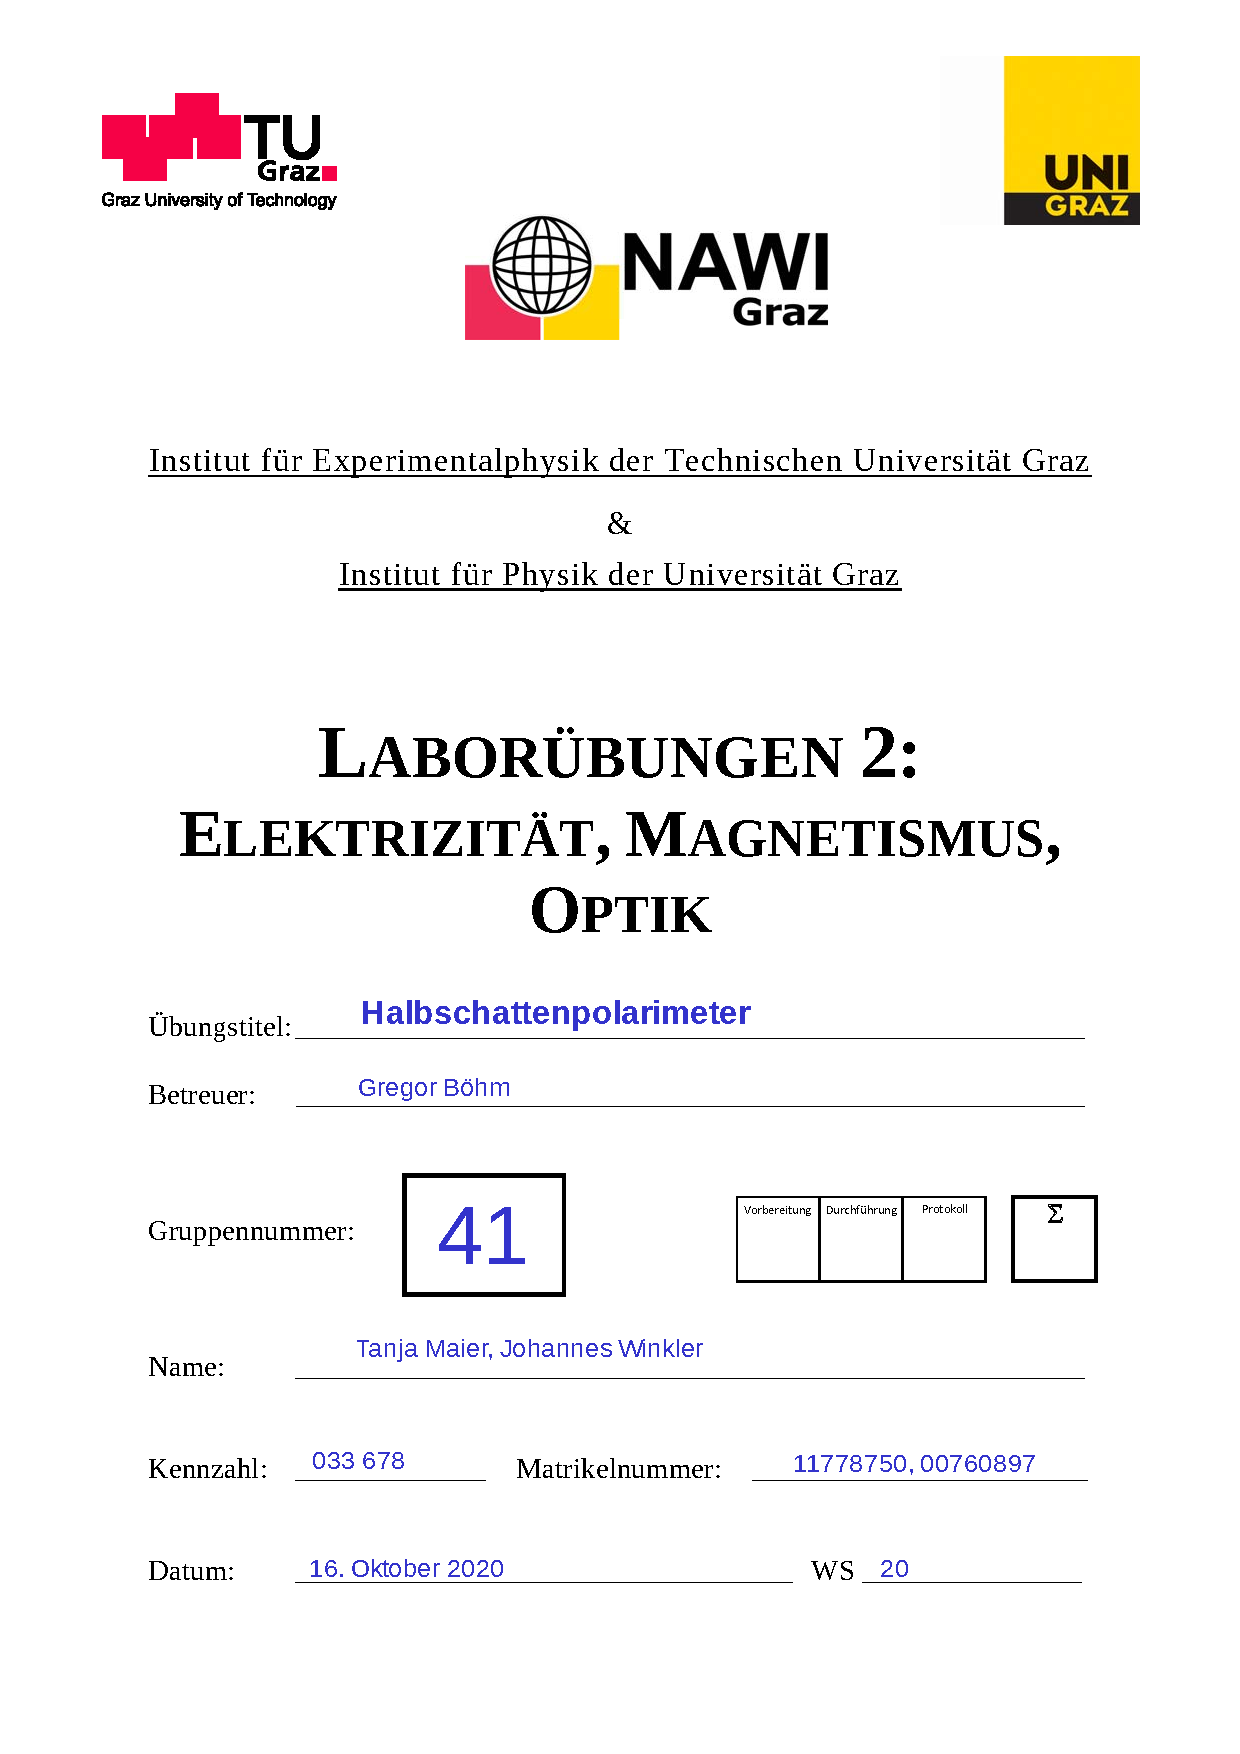
\includepdf{Deckblatt.pdf}


\pagestyle{fancy}

\section{Aufgabenstellung}

\begin{enumerate}
\item Bestimmung der Konzentration einer Rohrzuckerlösung.
\item Bestimmung der spezifischen Drehung einer Quarzplatte.
\end{enumerate}

\section{Grundlagen und Versuchsaufbau}

Unter optischer Aktivität versteht man die Eigenschaft mancher Medien, die Schwingungsebene linear polarisierten Lichts nach rechts oder links zu drehen. Dieses Verhalten wird durch eine schraubenfömige Struktur des Kristallgitters (bei festen Stoffen) bzw. der Moleküle (bei Flüssigkeiten und Gasen) hervorgerufen. Denkt man sich die linear polarisierte Welle aus zweientgegengesetzt zirkular polarisierten Wellen zusammengesetzt, können die beiden Anteile in einem solchen Medium unterschiedliche Ausbreitungsgeschwindigkeiten besitzen. Sie treten daher aus dem Medium mit einer Phasendifferenz aus, und setzen sich zu einer linear polarisierten Welle mit gedrehter Polarisationsrichtung zusammen. Die Größe des Winkels $\alpha$ ist von der durchlaufenen Wegstrecke $d$ bzw. $\ell$, der spezifischen Drehung $\as$ und der Konzentration des Mediums $c$ abhängig.

\begin{equation}
\label{eq:main}
\begin{aligned}
  \alpha &= \as\cdot \ell \cdot c && \text{für Flüssigkeiten und Gase} \\
  \alpha &= \as\cdot d && \text{für Kristalle und Festkörper}
\end{aligned}
\end{equation}

Um aus natürlichem Licht linear polarisiertes zu erhalten, kann z.B. ein Nicol'sches Prismaverwendet werden. Es besteht aus einem geeignet ausgerichteten und geschnittenen doppelbrechenden Kristall. Dabei wird eintretendes unpolarisiertes Licht in zwei senkrecht zueinanderstehende linear polarisierte Anteile mit unterschiedlicher Ausbreitungsgeschwindigkeit aufgespalten. Durch Totalreflexion eines der beiden Anteile an einer Grenzfläche können die beiden Polarisationsanteile voneinander getrennt werden.

Da es aus physiologischen Gründen schwierig ist, eine Polarisator – Analysator – Anordnung aufmaximale oder minimale Helligkeit abzugleichen, wird für Messzwecke ein sog. Halbschattenpolarimeter (Abb. \ref{fig:halbschattenpolarimeter}) verwendet. Dabei wird nach dem Polarisator ein nur den halben Strahlengangbedeckendes zweites Nicol'sches Prisma eingesetzt, das um einen kleinen Winkel gegen den Pola-risator verdreht ist. Beim Durchstimmen des Analysators beobachtet man in dem nun geteiltenGesichtsfeld nacheinander ein Helligkeitsminimum in beiden Hälften. Befindet sich der Analysator genau senkrecht zum Symmetriewinkel zwischen Polarisator und Halbschattenprisma,erscheinen beide Gesichtsfeldhälften gleich hell. Die Trennlinie ist nicht sichtbar. Bei einer ge-ringen Abweichung von dieser Stellung wird eine der beiden Hälften sofort dunkler. Dadurch istein präziser Abgleich der Polarisator – Analysatorstellung möglich.


\begin{figure}[H]
\centering
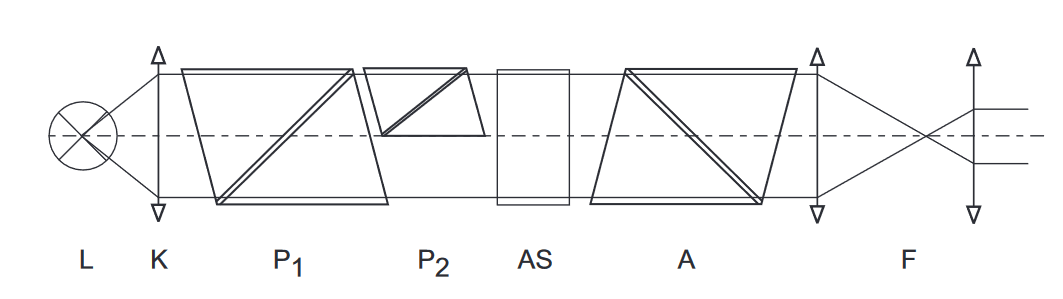
\includegraphics[scale=0.4]{halbschattenpolarimeter.png}
\caption{Aufbau des Halbschattenpolarimeters $L$ Na-Dampflampe, $K$ Kondensor, $P_1$ Polarisator, $P_2$ Halbschattenprisma, $AS$ optisch aktive Substanz, $A$ Analysator, $F$ Fernrohr}
\label{fig:halbschattenpolarimeter}
\end{figure}

\newpage

\section{Geräteliste}

\begin{table}[H]
\caption{Liste der verwendeten Geräte}

~

\begin{tabular}{l|llll}
Bezeichnung & Gerätenummer & Unsicherheit \\
\hline
Micrometer & & $\pm~0.01~$mm \\
1. Halbschattenpolarimeter & & $\pm~0.05~^\circ$ \\
2. Halbschattenpolarimeter & & $\pm~0.1~^\circ$ \\
Schiebelehre & & $\pm~0.05~$mm \\
Rohrzuckerlösung & & \\
Quarzkristalle & & 
\end{tabular}

\end{table}




\section{Durchführung und Messwerte}

\subsection{Rohrzuckerlösung}

Grundsätzlich müsste zuerst die Gesamtlänge des Probenglases mithilfe der Schiebelehre gemessen werden. Im Fall dieser Experimentdurchführung war die Länge des Probenglases jedoch schon angegeben und musste deshalb nicht mehr gemessen werden.

Die Länge des Probenglases betrug $\ell = 200~$mm und wurde als konstant angenommen.


Um die Größe des Winkels $\alpha$ zu bestimmen, musste der Halbschattenpolarimeter zunächst auf einen offset Winkel hin kalibriert werden. Dazu wurde der Übergang von \textit{hell-dunkel-hell} gesucht, das heißt der Punkt, an dem beide Anteile der Fläche gleich wenig Intensität aufweisen (also gleich dunkel sind) und gilt
\begin{align*}
A_1\cdot\cos(\alpha)\cdot\cos(\varphi-\alpha) = -A_1\cdot\cos(\alpha)
\end{align*}

Die Messung wurde fünf Mal wiederholt und in Tabelle \ref{tab:rohrzucker_offset_winkel} notiert.

\begin{table}[H]
\caption{Offset-Winkel für die Analyse der Rohrzuckerlösung.}
\label{tab:rohrzucker_offset_winkel}
\centering
\begin{tabular}{r|r}\\
 Nr. & $\alpha_\text{off}$ / ${}^\circ$  \\
 \hline
1 & 39.10\\
2 & 39.30\\
3 & 39.20\\
4 & 39.30\\
5 & 39.20\\
\hline \
 $\overline{x}$ & 39.22
\end{tabular}
\end{table}



Danach konnte das Probenglas in den Strahlengang eingelegt werden und der Winkel beim Übergang wurde erneut gemessen. Die Messung wurde zehn Mal durchgeführt und in Tabelle \ref{tab:rohrzucker_winkel} zusammengefasst.


\begin{table}[H]
\caption{Drehwinkel der Rohrzuckerlösung.}
\label{tab:rohrzucker_winkel}
\centering
\begin{tabular}{r|r}\\
 Nr & $\alpha_1$ / ${}^\circ$  \\
 \hline
1 & 26.20\\
2 & 25.20\\
3 & 26.60\\
4 & 25.50\\
5 & 25.30\\
6 & 26.30\\
7 & 26.50\\
8 & 26.10\\
9 & 25.50\\
10 & 26.60\\
\hline \
 $\overline{x}$ & 25.98
\end{tabular}
\end{table}


\subsection{Quarzkristalle}

Als erstes wurden die vier Quarzkristalle mithilfe einer Micrometerschraube jeweils zehn Mal vermessen. Die Werte sind in Tabelle \ref{tab:kristalle_dicken} zusammengefasst.

\begin{table}[H]
\caption{Dicken der Quarzkristalle.}
\label{tab:kristalle_dicken}
\centering
\begin{tabular}{rrrr}\\
 $d_1$ / mm & $d_2$ / mm & $d_3$ / mm & $d_4$ / mm  \\
 \hline
6.99 & 6.51 & 9.17 & 9.43\\
6.98 & 6.50 & 9.16 & 9.43\\
6.99 & 6.50 & 9.17 & 9.42\\
6.98 & 6.51 & 9.16 & 9.43\\
6.99 & 6.51 & 9.16 & 9.42
\end{tabular}
\end{table}


Dann wurde auch hier wieder zunächst der Halbschattenpolarimeter mithilfe des \textit{hell-dunkel-hell} Übergangs auf einen offset Winkel kalibriert und dann die Proben nacheinander eingelegt und wieder dieser Übergang gesucht. Die Messungen wurden sowohl für den offset Winkel als auch für die unterschiedlichen Quarzkristalle fünf Mal durchgeführt und in Tabelle \ref{tab:kristall_winkel} notiert.



\begin{table}[H]
\caption{Offset und Drehwinkel der Quarzkristalle.}
\label{tab:kristall_winkel}
\centering
\begin{tabular}{r|rrrr}\\
 $\alpha_\text{off}$ / ${}^\circ$ & $\alpha_1$ / ${}^\circ$ & $\alpha_2$ / ${}^\circ$ & $\alpha_3$ / ${}^\circ$ & $\alpha_4$ / ${}^\circ$  \\
 \hline
14.90 & 43.80 & 53.80 & -5.10 & 40.70\\
15.00 & 43.90 & 53.60 & -5.00 & 40.80\\
15.10 & 43.70 & 53.70 & -4.90 & 40.60\\
15.00 & 43.80 & 53.50 & -5.00 & 40.80\\
15.10 & 43.70 & 53.50 & -4.90 & 40.70
\end{tabular}
\end{table}


\section{Auswertung}


\subsection{Rohrzuckerlösung}


Bestimmung der Konzentration mit Gleichung \eqref{eq:main}, wobei die Länge $\ell$ und $\as$ als konstant angenommen wird.
\begin{align*}
c &= \frac{\alpha}{\as\cdot \ell} \\
\Delta c &= \frac{\Delta \alpha}{\as\cdot \ell}
\end{align*}
mit $\as = 66.5~\frac{{}^\circ\cdot \text{cm}^3}{\text{dm}\cdot \text{g}}$. Es ergibt sich
\begin{align*}\\
c = (99.55 \pm0.75)~\text{mg}/\text{cm}^3 \\
\end{align*}\\



\subsection{Quarzkristalle}

Hier wird tabellarisch ausgewertet mit der Formel
\begin{align*}
\beta_i = \frac{\overline{\alpha_i-\alpha_{\text{off}}} + x}{\overline{d_i}}
\end{align*}
wobei die Notation mit dem obigen Querstrich für das arithmetische Mittel steht. $x$ ist ein Winkel aus der Menge $\{0, 180^\circ, -180^\circ, 360^\circ, -360^\circ\}$.


\begin{table}[H]
\caption{Auswertung der Drehwinkel.}
\label{tab:kristall_auswertung}
\centering
\begin{tabular}{rrrrr}\\
 $x$ / ${}^\circ$ & $\beta_1$ / ${}^\circ$ & $\beta_2$ / ${}^\circ$ & $\beta_3$ / ${}^\circ$ & $\beta_4$ / ${}^\circ$  \\
 \hline
$0~^\circ$ & 4.08 & 6.09 & 17.52 & 2.71\\
$180~^\circ$ & 29.84 & 33.76 & 37.16 & {\color{red} 21.80}\\
$-180~^\circ$ & {\color{red} -21.68} & {\color{red} -21.58} & -2.13 & -16.38\\
$360~^\circ$ & 55.60 & 61.43 & 56.80 & 40.90\\
$-360~^\circ$ & -47.44 & -49.26 & {\color{red} -21.77} & -35.47
\end{tabular}
\end{table}


Die rot markierten Werte sind näherungsweise mit dem gegebenen Literaturwert vergleichbar. Daher wird von diesen Werten der betragsmäßige Mittelwert und die Standardabweichung berechnet. Dadurch ergibt sich als Ergebnis für den Drehwinkel von Quarz 
\begin{align*}\\
 \beta = (21.71 \pm 0.10)~^\circ\\
\end{align*}



\section{Diskussion}
Der Versuch wurde hier mit zwei unterschiedlichen Halbschattenpolarimetern durchgeführt, was die unterschiedlichen offset Winkel der jeweiligen Experimentteile bzw. die unterschiedlichen Unsicherheiten der beiden Geräte erklärt.
Der Drehwinkel von Quarz stimmt gut mit dem gefundenen Literaturwert [1] überein. Aufgrund des Vorzeichens und weil $\alpha$ kann man auch sagen, dass Quarz ein rechtsdrehendes Material ist [2].
Da die Konzentration der Zuckerlösung im Verhältnis zur beigegebenen Zuckermenge variiert, konnte hier mit keinem Literaturwert verglichen werden.



\section{Zusammenfassung}
Die Konzentration der Rohrzuckerlösung beläuft sich mit Fehler auf
\begin{align*}\\
c = (99.55 \pm0.75)~\text{mg}/\text{cm}^3 \\
\end{align*}\\


Der Drehwinkel von Quarz beläuft sich mit Fehler auf
\begin{align*}\\
 \beta = (21.71 \pm 0.10)~^\circ\\
\end{align*}


%\newpage 
%\appendix
%\section{Python Skript}



\definecolor{commentgreen}{RGB}{2,112,10}
\definecolor{eminence}{RGB}{108,48,130}
\definecolor{weborange}{RGB}{255,165,0}
\definecolor{frenchplum}{RGB}{129,20,83}

\lstdefinelanguage{python}{
    morekeywords={def, for, range, abs, return},
    otherkeywords={<-,->, |>, \%\{, \}, \{, \, (, )},
    sensitive=true,
    morecomment=[l]{\#},
    morecomment=[n]{/*}{*/},
    morecomment=[s][\color{purple}]{:}{\ },
    morestring=[s][\color{orange}]"",
    commentstyle=\color{commentgreen},
    keywordstyle=\color{eminence},
    stringstyle=\color{red},
	basicstyle=\ttfamily,
	breaklines,
	showstringspaces=false,
	frame=tb
}
%\lstinputlisting[language=Python,captionpos=b, label=lst:test,caption={Laplace Auswertung}]{generate_numbers_laplace.py}

%\lstinputlisting[language=Python,captionpos=b, label=lst:test,caption={Bessel Auswertung}]{generate_numbers_bessel.py}


%\lstinputlisting[language=Python,captionpos=b, label=lst:test,caption={Zerstreuungslinse Auswertung}]{generate_numbers_zerstreuungslinse.py}




\end{document}
